\chapter{\LaTeX: Making Beautiful Documents}\label{ch:latex}
% Goal: 40 pages

\section{Why \LaTeX?}
\index{latex}
We all have to write documents from time to time, be it a CV, a scientific article, a slideshow presentation or a school assignment. While knowing a professional typesetting tool such as \LaTeX{} may not be strictly necessary to do this, the outcome will almost certainly look more professional if you do.

\index{WYSIWYG}
Whether you are writing articles in Microsoft Word or LibreOffice Writer, or making a slideshow presentation in Microsoft PowerPoint or LibreOffice Impress, the focus is to a large extent on how stuff looks (what-you-see-is-what-you-get --- WYSIWYG). You as the author are often left with the responsibility of tweaking such typographic details as placement, font, text size, margins, etc. Unless you're schooled in typography, chances are you'll make a lot of mistakes which may seem subtle, but which is the difference between poor and professional typesetting.

With \LaTeX{} on the other hand, the writer focuses on what stuff \emph{is} and \LaTeX{} will take care of how stuff \emph{looks}. You may for instance declare that something is a title or a paragraph, but you do not get to typeset it. You may choose to emphasize a word, but \LaTeX{} chooses how (e.g. underlined, italic, bold, etc.). While it may feel unfamiliar at first that \LaTeX{} takes control of the looks of your document, it ensures a high typographic standard. Try to not to insist on having \LaTeX{} do things your way. There's usually a good reason it works the way it does.

The downside of declaring what stuff \emph{is}, is that it has to be done using code, and consequentially, there's a steeper learning curve. Indeed, you will probably spend more time writing documents as you start out with \LaTeX{} than you did previously, but you will also achieve nicer results. As you gain more experience, you may find that you don't even spend significantly more time writing in \LaTeX{} than in WYSIWYG tools, you just spend your time differently. Rather than tweaking typographic details manually, you will spend time looking for just the right \LaTeX{} command.

%Most people need to write text documents from time to time, be it a CV, an article or a school assignment. Especially if you're writing something you'll use in your profession, you likely want it to \emph{look} professional which usually is not the case when you use tools like Microsoft Word or LibreOffice Writer. With these what-you-see-is-what-you-get (WYSIWYG) tools, the author spends time manually tweaking how stuff looks; where the title is, which fonts to use, text sizes, and placement. Most of us are not interested enough in typography to do this right. In comparison, using \LaTeX{}, the writer focuses on what stuff \emph{is}, rather than how stuff \emph{looks}. By telling \LaTeX{} ``this is a title'', or ``this is a new paragraph'' \LaTeX{} itself will figure out the proper formatting. It may seem unfamiliar at first that \LaTeX{} decides how stuff looks, indeed many novices try to force \LaTeX{} to display stuff in a particular way. My advice: don't!

%\LaTeX{} certainly comes with a higher learning barrier before you can use it than WYSIWYG tools, but once you get familiar with it, I think you'll find that using it actually isn't that much slower, and it produces much better results. You may find a shift in what you spend time on: less time manually placing stuff, more time looking for how to do ``this thing'' with \LaTeX{} on the internet.

While there are other typesetting tools out available, \LaTeX{} is one of the most widely used, especially in scientific circles. \LaTeX{} is also based on \TeX{} which is developed by the computer science pioneer Donald Knuth, who is famous for having few bugs in his programs. If there should be one typesetting tool in your toolbox it has to be \LaTeX{}.

%Other professional typesetting tools exist as well, but \LaTeX{} is very well developed and by far the most widespread, at least in scientific publications and books. We'll also see how to use it for making slideshow presentations, thus replacing tools such as Microsoft PowerPoint. If there's one typesetting tool you want in your toolbox to it's definitely \LaTeX{}.

\section{Which Tools You Need}
\index{highlighting}
\index{Texmaker}
\LaTeX{} can be written in any plain text editor (like Notepad if you're using Windows) and stored to a file ending with .tex. The .tex file is then \emph{compiled} to generate a .pdf file using the command line tool \verb|pdflatex|. However, most users prefer a more specialized text editor which runs \verb|pdflatex| for you. Most such editors also supports highlighting, i.e.\ the application of different colors to different parts of the code to make it more readable. Many good editors exist, but we will use Texmaker which works on both Linux, OS X and Windows.

To get \LaTeX{}, you need to install a \LaTeX{} distribution. There are several of them, but the code you write is the same for all of them. Proceed according to your operating system to install a \LaTeX{} distribution and Texmaker.

\paragraph{Linux}
\index{TeX Live}
On Linux, TeX Live is the recommended distribution. On Debian-based Linuxes such as Ubuntu or Mint, you can install TeX Live and Texmaker using the following command:
\begin{verbatim}
$ sudo apt-get install texlive-full texmaker
\end{verbatim}

\paragraph{OS X}
\index{MacTeX}
For OS X, MacTeX is the recommended distribution. It is essentially the same as TeX Live but adds some compatibility to OS X. Download and install MacTeX and Texmaker from the following links:

~\\
\urlone{http://tug.org/mactex}
\urlone{http://www.xm1math.net/texmaker}

\paragraph{Windows}
\index{MiKTeX}
For Windows either TeX Live or MiKTeX can be used, but many find MiKTeX slightly easier to handle. Install MiKTeX and Texmaker from the following links:

~\\
\urlone{http://www.miktex.org}
\urlone{http://www.xm1math.net/texmaker}

It is also useful to know a program or two with which you can make nice illustrations and images for your documents. Since this is not coding it falls outside the scope of this book. A few recommendations are made though, to complement your knowledge in \LaTeX.  

An excellent tool for making illustrations is InkScape. Gimp is also useful, in particular for photos, but it is not as suited for illustrations as InkScape. They can be installed as follows:

\paragraph{Linux} Run:
\begin{verbatim}
$ sudo apt-get install gimp inkscape
\end{verbatim}

\paragraph{OS X and Windows}
Download and install from:

~\\
\urlone{http://inkscape.org}
\urlone{http://www.gimp.org}

If you plan to use text labels inside your illustrations you may also want to download the font used by \LaTeX{}, Computer Modern, but we'll get back to this.


\section{Hello World!}
We will start by going through \reflst{latex:minimal} which is about the minimum code required to start a new document. The left part is the source code while the right part demonstrates the output produced by the code. The actual result will necessarily be slightly different, since it will be placed in its own document with its margins and formatting, but a demonstration may be instructive nonetheless.

\begin{listing}
	\rule{\textwidth}{0.4pt}
	\begin{minipage}[t]{0.49\textwidth}
		\inputminted[frame=none]{latex}{latex/first.tex}
	\end{minipage}\hfill\vline\hfill
	\begin{minipage}[t]{0.49\textwidth}
		Hello World!
	\end{minipage}\\[0.5em]
	\rule{\textwidth}{0.4pt}
	\caption{A (near-)minimal \LaTeX{} document}
	\label{lst:latex:minimal}
\end{listing}

\index{command}
\index{argument}
\index{option}
Notice that all \LaTeX{}-\emph{commands} start with a backslash, and may be followed by mandatory \emph{arguments} in curly braces, and optional arguments (\emph{options}) in square brackets like this:

\index{syntax}
\latexone|\command[option1,option2]{argument1}{argument2}|
\noindent Such ``rules'' for how commands are structured is usually referred to as \emph{syntax}.

\index{\latexin{\documentclass}}
The first command in any document is \latexin{\documentclass} which tells \LaTeX{} what kind of document it is. Some possible arguments are shown in \reftab{latex:documentclass}. The option \latexin{a4paper} tells \LaTeX{} to produce a document in paper size A4. \latexin{\documentclass} also support options for other paper sizes, font sizes, etc.\ which you can find on the internet whenever you need it.

\begin{table}
	\centering
	\caption{Document classes}
	\begin{tabular}{ll}
	\hline
	\latexin{book}		&	For books.																\\
	\latexin{report}		&	For reports and somewhat big documents (tens of pages).					\\
	\latexin{article}	&	For articles and smaller documents. Excludes chapters.					\\
	\latexin{letter}		&	For letters.																\\
	\latexin{beamer}		&	For	slideshow presentations using the Beamer package.						\\
	\latexin{curve}		&	For CVs using the Curve package.
	\end{tabular}
	\label{tab:latex:documentclass}
\end{table}

\index{\latexin{\usepackage}}
\index{\latexin{inputenc}}
\index{\latexin{fontenc}}
\index{\latexin{babel}}
\index{package}
\index{font encoding}
\index{character encoding}
Next, the functionality of \LaTeX{} can be expanded by including \emph{packages} which provides more features (similar to \emph{modules} in Python or \emph{libraries} in other languages). This is done by the \mintinline{latex}{\usepackage} command, one per package you want to use. To begin with, we need three packages: \latexin{inputenc} specifies the \emph{character encoding} which is used in the .tex files. We'll get back to this. \mintinline{latex}{fontenc} determines the \emph{font encoding} to be used in the .pdf-file. We won't dig into this but it should usually be T1. Finally, \mintinline{latex}{babel} specifies the written language.

\index{environment}
\index{\latexin{\begin}}
\index{\latexin{\end}}
\index{comment}
The next new thing we'll encounter is an \emph{environment}. An environment starts with a \latexin{\begin} and ends with an \latexin{\end}, and affects anything in between. The \latexin{document} environment is where you write what actually goes into the document. Here, the only thing in the document is the text ``Hello World!''. Text is written straight forward, with a few exceptions which we'll get back to. When \LaTeX{} encounters a \% character, it ignores anything on the rest of that line. This is known as a \emph{comment} and is only visible in the source code. You may use comments to explain things which is not obvious in the source code for later reference.

\index{preamble}
The part between \latexin{\documentclass} and \latexin{\begin{document}} which is used to load packages, and make other configurations to the document is known as the \emph{preamble}.

\subsection{Character Encoding}
\index{character encoding}
\index{ASCII}
\index{UTF-8}
Whenever text is stored in a file it is represented by strings of zeros and ones (\emph{binary digits} or just \emph{bits}) according to a \emph{character encoding standard}. An early standard is the \emph{ASCII} standard (American Standard Code for Information Interchange) which uses 7 bits to represent letters. For instance, ``A'' is represented by the binary number 1000001 which maps to 65 when converted to the decimal system. Since 7 bits can only encode 128 characters, only the most common characters were included in the ASCII standard. By expanding it with one bit, 128 characters more could be encoded. However, this is still not enough for all kinds of languages, and as a result, different 8 bit encodings exist depending on where you're from. One of the most popular is ISO-8859-1 which includes the letters used in Western European languages. However, then you cannot use letters outside of this standard. UTF-8 (Unicode Transformation Format, 8-bit), on the other hand, is a very clever encoding which circumvents this problem by using 8 bits (or one byte) for the most common characters but may use up to four bytes for rarer characters. As such, UTF-8 has a wide range of characters and should cover all your needs while not making the text documents much larger. I recommended storing all .tex files as UTF-8 to avoid encoding problems.

In Texmaker you can ensure files are stored as UTF-8 by going to Options$\rightarrow$ Configure Texmaker (see \reffig{latex:texmaker}), open the ``Editor'' pane and make sure ``Editor Font Encoding'' is set to UTF-8. Finally, the \LaTeX{} compiler needs to know the encoding to decode it correctly as well. This is what we've told it in the option for the \latexin{inputenc} package in \reflst{latex:minimal}. A common pitfall is that the \latexin{inputenc} option does not match the actual encoding used in the file which causes local/special (non-ASCII) characters to look like other symbols.

\begin{figure}
	\centering
	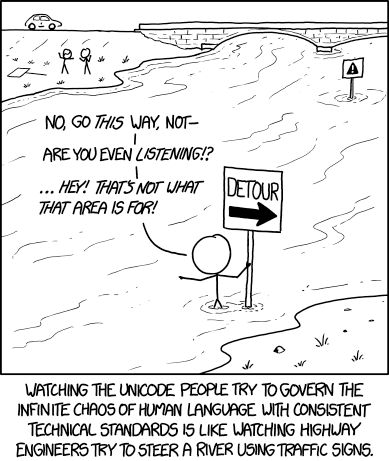
\includegraphics[scale=1,resolution=150]{graphics/unicode.png}
	\caption{It can sometimes be hard to convince people to use UTF-8. ``Unicode'' (\url{https://xkcd.com/1726}) by Randall Munroe is licensed under \mbox{CC~BY-NC~2.5}.}
	\label{fig:latex:unicode}
\end{figure}

\subsection{Compiling}\label{sec:latex:compiling}
\index{compilation}
\index{\verb|latex|}
\index{\verb|pdflatex|}
The next step is to compile our minimal example to turn it into a .pdf file. The minimal example from \reflst{latex:minimal} can be saved to a UTF-8 encoded file \texttt{main.tex} in a new folder. You \emph{do} want to create a separate folder for each document you write since \LaTeX{} generates lots of other files in this folder upon compilation.

One should be aware that people use different compilation strategies. Some people use the program \texttt{latex} which generates a .dvi file and then converts it to .pdf using a conversion tool, while we will use the program \texttt{pdflatex} which directly generates the .pdf file. Both of these are command line programs but Texmaker can run these commands so we don't have to. However, to better grasp what's going on behind the curtains, we will see how it's done both from the command line and from Texmaker. If you haven't read \refch{bash} yet, don't worry. You don't need to be able to run the commands to proceed this chapter.

\paragraph{Using the Command Line}
To compile \texttt{main.tex} using the (Linux, OS X or Windows) command line, navigate to the folder where the file is, and simply run:
\begin{verbatim}
$ pdflatex main.tex
\end{verbatim}
and a file named \verb|main.pdf| will be created. If you got no errors you're done.

But computers are very literal and errors is the most common thing. If there's a typo somewhere in your code, e.g. a capital letter instead of a small one in a command, the document simply will not compile, but returns an error. The error messages may look cryptic at first, but they do tell what the error is and which line it is on. You can exit the failed compilation in the command line by typing ``x''. Try to sort out one error at a time, starting with the top one.

Sometimes, when you have an error in your code, and you can't figure out what it is, it may be useful to \emph{comment out} a block of lines. Texmaker supports commenting out multiple lines by marking them and hitting Ctrl+T. Uncommenting the marked lines is done by Ctrl+U. Another advice: Compile your document often to avoid a bunch of errors to accumulate. Fixing errors is perhaps the largest barrier when starting to program, but it gets a lot easier with a little experience.

\paragraph{Using Texmaker}
Next: compile using Texmaker. We can use the arrow next to the ``Quick Build'' drop down menu (see \reffig{latex:texmaker}) to run any of the programs available from the drop down menu. As an example, we can choose ``PDFLaTeX'' and click the arrow, and to view it, we can click the arrow next to ``View PDF''. The ``Quick Build'' option is useful, since it can be configured to run a series of commands in sequence. If you again go to Options$\rightarrow$Configure~Texmaker and select the ``Quick Build'' pane you can set Quick Build to ``PdfLaTeX + View PDF''. In the ``Commands'' pane, you can see exactly which commands Texmaker uses when running this programs. These are fine as they are. Now, when you choose ``Quick Build'' and click the arrow, the document will be compiled and displayed. Like when using the command line errors must be resolved to make the document compile.

\begin{figure}
	\centering
	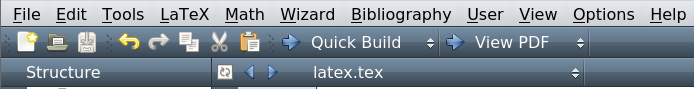
\includegraphics[width=\textwidth]{graphics/texmaker.png}
	\caption{Texmaker toolbar}
	\label{fig:latex:texmaker}
\end{figure}

To build actual skills one must practice and not just read about coding. It does not have to take much time if you only want to master the basics (which is a start), but some practice is an absolute necessity. To help you with this we sometimes provide suggested exercises, some of which have suggested answers in \refch{answers}. It's up to you if you want to do the exercises or if you want to find other means of practicing. It may also be a good idea to try out examples as you go. Perhaps the best practice, though, are real-world examples, so if you have any project, don't hesitate. That's the kind of practice which makes perfect!

\section{Exercises}
\begin{ExerciseList}
	\Exercise Create (in a new folder) a \verb|main.tex| file looking like \reflst{latex:minimal} and compile.
\end{ExerciseList}

\section{Writing Text}\label{sec:latex:writing}
\index{reserved characters}
As previously mentioned, writing text in \LaTeX{} is \emph{mostly} straight forward, but there are some things you need to pay attention to. First up are the \emph{reserved characters} listed in \reftab{latex:reserved}. These characters have special meanings i \LaTeX{}, for instance ``\%'' starts a comment, and must therefore be written using a command. Consider this example:

\latexone{We offer a mortgage at 5% interest.}
\noindent Here the last character printed is ``5'' since the rest is a comment. The proper way to write this would be

\latexone{We offer a mortgage at 5\% interest.}

%\begin{table}
%	\centering
%	\caption{Reserved Characters}
%	\begin{tabular}{ll}
%	\hline
%	\latexin{\#}					&	\# 		\\
%	\latexin{\$}					&	\$		\\
%	\latexin{\%}					&	\%		\\	
%	\latexin{\&}					&	\&		\\
%	\latexin{\_}					&	\_		\\
%	\latexin|\{|					&	\{		\\
%	\latexin|\}|					&	\}		\\
%	\latexin{\^{}}				&	\^{}		\\
%	\latexin{\~{}}				&	\~{}		\\
%	\latexin{\textbackslash{}}	&	\textbackslash
%	\end{tabular}
%	\label{tab:latex:reserved}
%\end{table}

\begin{table}
	\centering
	\caption{Reserved Characters}
	\begin{tabular}{l m{3cm} l l}
	\hline
	\latexin{\#}					&	\# 		&	\latexin|\{|					&	\{		\\
	\latexin{\$}					&	\$		&	\latexin|\}|					&	\}		\\
	\latexin{\%}					&	\%		&	\latexin{\^{}}				&	\^{}		\\
	\latexin{\&}					&	\&		&	\latexin{\~{}}				&	\~{}		\\
	\latexin{\_}					&	\_		&	\latexin{\textbackslash{}}	&	\textbackslash
	\end{tabular}
	\label{tab:latex:reserved}
\end{table}

%\begin{table}
%	\centering
%	\caption{Reserved Characters}
%	\begin{tabular}{cccccccccc}
%	\hline
%	\latexin{\#}	& \latexin{\$}	& \latexin{\%}	& \latexin{\&}	& \latexin{\_}				&
%	\latexin|\{|	& \latexin|\}|	& \latexin{\^{}}	& \latexin{\~{}}	& \latexin{\textbackslash{}}	\\
%	\#			& \$				& \%				& \&				& \_							&
%	\{			& \}				& \^{}			& \~{}			& \textbackslash{}
%	\end{tabular}
%	\label{tab:latex:reserved}
%\end{table}

Next, quotations (in American English) are written starting with two backticks and ending with two apostrophes,

\latexone{``What's up?'' said George.}
\noindent The backticks and apostrophes will be replaced by proper quotation marks. Just using \latexin{"} is incorrect. If you need nested quotations, use a single backtick and apostrophe for the inner quote:

\latexone{``George asked me `what's up'.''}
\noindent This will evaluate to

\begin{quote}
``George asked me `what's up'.''
\end{quote}
Beware though that different languages use different conventions, e.g. French quotes are written like <<this>> (\latexin{<<this>>}) while German are written like ,,this'' (\latexin{,,this''}). Make sure you use the style according to your language\footnote{\url{https://en.wikipedia.org/wiki/Quotation_mark}}.

\index{hyphen}
\index{en-dash}
\index{em-dash}
\index{minus}
Next, let's learn to distinguish between hyphens and different kinds of dashes. \emph{Hyphens} are used for joining words. \emph{En-dash} is used when talking about numbers in a range, e.g.\ the years 1980--1990, and \emph{em-dash} is used as punctuation---for instance like this---in a sentence. See \reftab{latex:dashes} for examples of how to use them. Hyphens and dashes should not be used for minus. Minus is written using math mode (\refsec{latex:equations}).

\begin{table}
	\centering
	\caption{Hyphen, dashes and minus}
	\begin{tabular}{llll}
	\hline
	Hyphen	&	\latexin{mother-in-law}					&	mother-in-law							\\
	En-dash	&	\latexin{pages 3--7}						&	pages 3--7								\\
	Em-dash	&	\latexin{``Let's see---15 euros''}		&	``Let's see---15 euros''		\\
	Minus	&	\latexin{The answer is $-4$}				&	The answer is $-4$
	\end{tabular}
	\label{tab:latex:dashes}
\end{table}

\index{\latexin{\emph}}
\index{\latexin{\em}}
To emphasize part of a text use the command \latexin{\emph}, for instance

\latexone{This is \emph{very} important!}
\noindent which becomes

\begin{quote}
	This is {\em very} important!
\end{quote}
An equivalent way of writing this is:

\latexone{This is {\em very} important!}

\index{switch}
\index{scope}
The difference between \latexin{\emph} and \latexin{\em} is that the latter is a \emph{switch} which means that it takes no arguments, but rather changes the style of the current \emph{scope}. The scope is here limited by \{ and \} so the switch \latexin{\em} only applies to the word ``very''. Environments also limits scope. The outermost scope is the \latexin{document} environment, so unless you limit the scope somehow you will emphasize the rest of the document. While it is advised you stick with \latexin{\emph} it is useful to know that commands often have a switch variant doing the same thing.

Emphasized text normally appear italic, that is, slanted and with more calligraphically styled letters. You can also directly specify that text should be for instance \underline{underlined}, using commands from \reftab{latex:formatting}. However, you normally should not do that. Remember, you tell \LaTeX{} what stuff \emph{is} and \LaTeX{} takes care of how stuff \emph{looks}. Italic is also subtler than the alternatives and in my opinion this looks better. Just look at how the \underline{underlined} words on this page damages the aesthetics of the whole page! You don't need to notice that a word is emphasized until you're actually reading it.

Furthermore, what if you want to emphasize a word inside something that's already emphasized? \latexin{\emph} takes care of this too:

\begin{quote}
I said, \emph{this is \emph{very} important!}
\end{quote}

\begin{table}
	\centering
	\caption{Formatting}
	\begin{tabular}{ll}
	\hline
	\latexin{\textrm{Roman}}			&	\textrm{Roman}		\\
	\latexin{\textbf{Bold}}			&	\textbf{Bold}		\\
	\latexin{\textsl{Slanted}}		&	\textsl{Slanted}		\\	
	\latexin{\textit{Italic}}		&	\textit{Italic}		\\
	\latexin{\textsc{Small Caps}}		&	\textsc{Small Caps}	\\
	\latexin{\textsf{Sans Serif}}		&	\textsf{Sans Serif}	\\
	\latexin{\texttt{Teletype}}		&	\texttt{Teletype}	\\
	\latexin{\underline{Underlined}}	&	\underline{Underlined}
	\end{tabular}
	\label{tab:latex:formatting}
\end{table}

\section{Document Structure}
\index{\latexin{\chapter}}
\index{\latexin{\section}}
\index{\latexin{\subsection}}
\index{\latexin{\subsubsection}}
A new chapter is started using the \latexin{\chapter} command, with the name of the chapter as its argument. Chapters can be split into \emph{sections} using the \latexin{\section} command, which again can be split into \emph{subsections} (\latexin{\subsection}) and further on to \emph{subsubsection} (\latexin{\subsubsection}). See \reflst{latex:structure} for an example. Numbering of chapters, sections and so on happen automatically.

\begin{listing}[H]
	\inputminted[frame=lines,linenos]{latex}{latex/structure.tex}
	\caption{A \LaTeX{} document with some structure and text}
	\label{lst:latex:structure}
\end{listing}

A chapter is a rather big, voluminous entity. The chapter's title may well consume approximately half a page, like in this book. In smaller documents like articles, school assignments, etc., which may only be a few pages long, this is not appropriate. The  \latexin{article} document class is suitable in such cases since it does not have chapters. There, sections are the highest structural level.

Further on, \LaTeX{} do not care if you write a whole paragraph in one line, or split it up into more lines. It will not break the lines where you do, but where it deems appropriate. Different paragraphs are separated by an open line (line 25 in \reflst{latex:structure}). 

\subsection{Table of Contents}
\index{\latexin{\tableofcontents}}
Due to \LaTeX{}'s awareness of contents, it can also auto-generate a table of contents for you. This is done with the \latexin{\tableofcontents} command on line 8. When compiling the document, \LaTeX{} makes a list of all the chapters and sections and then stores it in a file. Upon next compilation, when it encounters \latexin{\tableofcontents}, this list will be used to make the table of contents. Unfortunately, if you did any changes to the ordering of the chapters in between, this list is now outdated, and the table of contents is incorrect. This behavior is typical for \LaTeX{}, which stores auxiliary information in files after compilation. To remedy this, compile the document again.

\subsection{Splitting Documents into Several Files}
As your document gets bigger, your \verb|main.tex| file may start looking like a mess and you just can't find the parts your looking for. In such cases, it is very useful to split the document into multiple files, for instance one file per chapter, section or any other appropriately sized chunks of text. Another benefit of this is that it gets easier to collaborate with others on the document. For instance, if you and your friend work on separate chapters, you can work on separate files.

\begin{listing}
	\inputminted[frame=lines,linenos]{latex}{latex/multifiles.tex}
	\caption{A .tex file with chapters in separate subfiles}
	\label{lst:latex:multifiles}
\end{listing}

\reflst{latex:multifiles} shows a new \verb|main.tex| file which uses the \latexin{\input} command to load the contents of other files. If you use \latexin{\chapter{Introduction}
Programmers, engineers, scientists and tech-savvy people in general have had the opportunity to learn a bunch of different computer programs and programming languages which makes their everyday work in front of the computer both easier and more efficient. In comparison, less technically oriented people, who lack such a toolbox, often end up using inconvenient tools and therefore end up using inefficient and impractical solutions.

Consider for instance that you have hundreds of photos and you’d like to change the resolution on all of them? Or maybe add a watermark before sharing them? Or change the filename to include the date? Such tasks can be tedious if you don’t know the right tools. However, the file names of all files can be changed using a single command in the Bash command line interface. A script that adds a watermark to every image takes less then 20 lines of code using the Python scripting language. Of course, programming takes time to learn, and it’s not for everybody to become a full time professional programmer. But with the emergence of modern low-threshold scripting languages like Python, why should such handy techniques still be reserved for geeks only?

Another thing which many may benefit from is learning a professional typesetting tool like LaTeX to write documents. Applications, CV’s, reports, slideshows, etc. Because let’s admit it: Most of us aren’t typographists. We don’t know exactly which font to use, which size, which line spacing and which margins to use everywhere to make a document look professional. LaTeX takes care of all that for you, but then you need to tell LaTeX what’s supposed to be a chapter, what’s a new paragraph, and so on. And that’s done by coding. It doesn’t have to be that hard, to start a new chapter with the title “Introduction”, for instance, you simply type 

\latexone{\chapter{Introduction}}
And how do you generate a table of contents in LaTeX? Simple. Because LaTeX know what the chapters are, all you have to do is type:
\latexone{\tableofcontents}
where you want your table of contents.

And as a last example, have you ever had to collaborate with someone to write a document in a normal text processing tool such as Microsoft Word? Then you’ll know it’s a mess. No two people can edit the document at once, despite editing different parts of the file. Documents written in LaTeX, as well as programs written in languages such as Python can be efficiently shared amongs many users using a Version Control System (VCS) such as Git and everyone can work on it simultaneously without stepping on each other’s toes! VCSs like Git also allows you to backtrack the whole history of your documents in case you regret something you once did.

The aim of this little book is to provide the normal guy on the street with at least a small toolbox allowing him or her to work more efficiently. More in a similar manner as professionals. The tools presented are carefully selected because together, they form a minimal toolbox allowing the reader to use a computer in such a rich way. Moreover, they are considered to be more useful, versatile and simple to learn than other alternatives. Admittedly, we will only scratch the surface of all these tools. Just enough to get you started, with pointers of where to look for further information. True, it will not even cover the same depth as most beginner’s books, since it is not the aim of this book to turn you into a programmer. However, it is assumed that the reader, being a generation which has grown up with technology, is capable of finding his/her way around in simple graphical computer programs. Therefore this book will focus on the coding aspects, only providing pointers to which graphical programs may be useful (for instance to make figures in documents).

Finally, each part are self-contained and may be read independently of the other parts (although using Git is kind of meaningless without knowing some other coding).} or simply \latexin{\chapter{Introduction}
Programmers, engineers, scientists and tech-savvy people in general have had the opportunity to learn a bunch of different computer programs and programming languages which makes their everyday work in front of the computer both easier and more efficient. In comparison, less technically oriented people, who lack such a toolbox, often end up using inconvenient tools and therefore end up using inefficient and impractical solutions.

Consider for instance that you have hundreds of photos and you’d like to change the resolution on all of them? Or maybe add a watermark before sharing them? Or change the filename to include the date? Such tasks can be tedious if you don’t know the right tools. However, the file names of all files can be changed using a single command in the Bash command line interface. A script that adds a watermark to every image takes less then 20 lines of code using the Python scripting language. Of course, programming takes time to learn, and it’s not for everybody to become a full time professional programmer. But with the emergence of modern low-threshold scripting languages like Python, why should such handy techniques still be reserved for geeks only?

Another thing which many may benefit from is learning a professional typesetting tool like LaTeX to write documents. Applications, CV’s, reports, slideshows, etc. Because let’s admit it: Most of us aren’t typographists. We don’t know exactly which font to use, which size, which line spacing and which margins to use everywhere to make a document look professional. LaTeX takes care of all that for you, but then you need to tell LaTeX what’s supposed to be a chapter, what’s a new paragraph, and so on. And that’s done by coding. It doesn’t have to be that hard, to start a new chapter with the title “Introduction”, for instance, you simply type 

\latexone{\chapter{Introduction}}
And how do you generate a table of contents in LaTeX? Simple. Because LaTeX know what the chapters are, all you have to do is type:
\latexone{\tableofcontents}
where you want your table of contents.

And as a last example, have you ever had to collaborate with someone to write a document in a normal text processing tool such as Microsoft Word? Then you’ll know it’s a mess. No two people can edit the document at once, despite editing different parts of the file. Documents written in LaTeX, as well as programs written in languages such as Python can be efficiently shared amongs many users using a Version Control System (VCS) such as Git and everyone can work on it simultaneously without stepping on each other’s toes! VCSs like Git also allows you to backtrack the whole history of your documents in case you regret something you once did.

The aim of this little book is to provide the normal guy on the street with at least a small toolbox allowing him or her to work more efficiently. More in a similar manner as professionals. The tools presented are carefully selected because together, they form a minimal toolbox allowing the reader to use a computer in such a rich way. Moreover, they are considered to be more useful, versatile and simple to learn than other alternatives. Admittedly, we will only scratch the surface of all these tools. Just enough to get you started, with pointers of where to look for further information. True, it will not even cover the same depth as most beginner’s books, since it is not the aim of this book to turn you into a programmer. However, it is assumed that the reader, being a generation which has grown up with technology, is capable of finding his/her way around in simple graphical computer programs. Therefore this book will focus on the coding aspects, only providing pointers to which graphical programs may be useful (for instance to make figures in documents).

Finally, each part are self-contained and may be read independently of the other parts (although using Git is kind of meaningless without knowing some other coding).} it searches for a file \verb|introduction.tex| in the same folder as \verb|main.tex|. You can also specify subfolders, like\\ \latexin{\chapter{Introduction}
Programmers, engineers, scientists and tech-savvy people in general have had the opportunity to learn a bunch of different computer programs and programming languages which makes their everyday work in front of the computer both easier and more efficient. In comparison, less technically oriented people, who lack such a toolbox, often end up using inconvenient tools and therefore end up using inefficient and impractical solutions.

Consider for instance that you have hundreds of photos and you’d like to change the resolution on all of them? Or maybe add a watermark before sharing them? Or change the filename to include the date? Such tasks can be tedious if you don’t know the right tools. However, the file names of all files can be changed using a single command in the Bash command line interface. A script that adds a watermark to every image takes less then 20 lines of code using the Python scripting language. Of course, programming takes time to learn, and it’s not for everybody to become a full time professional programmer. But with the emergence of modern low-threshold scripting languages like Python, why should such handy techniques still be reserved for geeks only?

Another thing which many may benefit from is learning a professional typesetting tool like LaTeX to write documents. Applications, CV’s, reports, slideshows, etc. Because let’s admit it: Most of us aren’t typographists. We don’t know exactly which font to use, which size, which line spacing and which margins to use everywhere to make a document look professional. LaTeX takes care of all that for you, but then you need to tell LaTeX what’s supposed to be a chapter, what’s a new paragraph, and so on. And that’s done by coding. It doesn’t have to be that hard, to start a new chapter with the title “Introduction”, for instance, you simply type 

\latexone{\chapter{Introduction}}
And how do you generate a table of contents in LaTeX? Simple. Because LaTeX know what the chapters are, all you have to do is type:
\latexone{\tableofcontents}
where you want your table of contents.

And as a last example, have you ever had to collaborate with someone to write a document in a normal text processing tool such as Microsoft Word? Then you’ll know it’s a mess. No two people can edit the document at once, despite editing different parts of the file. Documents written in LaTeX, as well as programs written in languages such as Python can be efficiently shared amongs many users using a Version Control System (VCS) such as Git and everyone can work on it simultaneously without stepping on each other’s toes! VCSs like Git also allows you to backtrack the whole history of your documents in case you regret something you once did.

The aim of this little book is to provide the normal guy on the street with at least a small toolbox allowing him or her to work more efficiently. More in a similar manner as professionals. The tools presented are carefully selected because together, they form a minimal toolbox allowing the reader to use a computer in such a rich way. Moreover, they are considered to be more useful, versatile and simple to learn than other alternatives. Admittedly, we will only scratch the surface of all these tools. Just enough to get you started, with pointers of where to look for further information. True, it will not even cover the same depth as most beginner’s books, since it is not the aim of this book to turn you into a programmer. However, it is assumed that the reader, being a generation which has grown up with technology, is capable of finding his/her way around in simple graphical computer programs. Therefore this book will focus on the coding aspects, only providing pointers to which graphical programs may be useful (for instance to make figures in documents).

Finally, each part are self-contained and may be read independently of the other parts (although using Git is kind of meaningless without knowing some other coding).}, although I normally prefer to keep all .tex files in the same folder.

\verb|introduction.tex| may for instance look like this:
%\begin{listing}
	\inputminted[frame=lines,linenos]{latex}{latex/introduction.tex}
%	\caption{A chapter put into a separate file}
%	\label{lst:latex:introduction}
%\end{listing}
Note that \verb|main.tex| still is the file you need to compile. Compiling e.g.\ \verb|introduction.tex| produces an error.

\section{Title Page}\label{sec:latex:title}
\index{\latexin{\maketitle}}
\index{\latexin{\title}}
\index{\latexin{\author}}
\index{\latexin{\date}}
\LaTeX{} is able to auto-generate a simple title page for you using the command \latexin{\maketitle}. To do that, it needs to know the title of the document, the author, and/or the date of publication. The commands \latexin{\title}, \latexin{\author} and \latexin{\date} can be put in the preamble to tell \LaTeX{} the title and author of the document, along with the date it was written/published. An example is shown in \reflst{latex:title}.

\begin{listing}
	\inputminted[frame=lines,linenos]{latex}{latex/title.tex}
	\caption{A .tex file with a title}
	\label{lst:latex:title}
\end{listing}

\index{\latexin{\today}}
But we can do better than what we did in \reflst{latex:title}, we can use \latexin{\date{\today}}. The command \latexin{\today} always inserts the date when the document is compiled, for instance, ``November 10, 2016''. The date format used by \latexin{\today} can be changed using the \latexin{datetime} package, e.g.\

\latexone{\usepackage[ddmmyyyy]{datetime}}
\noindent Now the date would show up as ``10/11/2016''. The default date separator, stored in the command \latexin{\dateseparator}, equals slash. I.e.\ typing \latexin{\dateseparator} is equivalent of writing a slash. We can redefine this command to be a period by inserting the following line somewhere in the preamble (between all the \latexin{\usepackage}'s and \latexin{\begin{document}}):

\latexone{\renewcommand{\dateseparator}{.}}
\noindent\latexin{\today} would now evaluate to ``10.11.2016''.

\index{Lorem Ipsum}

\section{Exercises}

\begin{ExerciseList}
	\Exercise Create (in a new folder) a \verb|main.tex| file looking like \reflst{latex:multifiles} along with files \verb|introduction.tex| and \verb|conclusion.tex| with a chapter and some dummy text. Compile \verb|main.tex|.
	\Exercise Add a titlepage, using \latexin{\today} to specify today's date.
	\Exercise Change the format of \latexin{\today} to 16.11.16.
	\Answer ~\\ \inputminted[frame=lines]{latex}{latex/exer_multi.tex}
	\Exercise Dummy texts like ``Contents in introduction chapter'' are not very good. Try replacing the contents in one of the chapters by this dummy text:
	
	\begin{quote}
			``Oh no! We need to write an awesomely nice document in 20--30 minutes---but \emph{how}?'' said George. ``Let's use \LaTeX{}'' replied Lisa.
	\end{quote}
	
	Hint: You may need to use the command \latexin{\LaTeX{}}.
	\Answer ~\\
	\begin{minted}{latex}
		``Oh no! We need to write an awesomely nice document
		in 20--30 minutes---but \emph{how}?'' said George. 
		``Let's use \LaTeX{}'' replied Lisa.
	\end{minted}
	You could also have used just \latexin{\LaTeX} instead of \latexin{\LaTeX{}} in this example. However, beware that writing \latexin{\LaTeX} followed by a space is equivalent of writing \latexin{\LaTeX{ }}, so it eats up the space between words.
	\Exercise Change the language of the document to your native tongue. Use the internet to find the right option of the \latexin{babel} package. Hint: When you change the language of the babel package of an already existing document you need to delete the file \verb|main.aux| before compiling. This is because \verb|main.aux|, which is an auxiliary file \LaTeX{} uses, remembers the previously used language and this causes a conflict in the compiler. This is a common pitfall.
	\Exercise Use the web to find the correct quotation marks for your native tongue and translate the above dialogue as well.
	\Exercise Even better is the standard dummy text \emph{Lorem Ipsum} using the \latexin{\lipsum} command. You can either use just \latexin{\lipsum} or optionally, \latexin{\lipsum[2-4]} to print, in this case, paragraphs 2--4 of the Lorem Ipsum text. \latexin{\lipsum} is not built into \LaTeX{} but is provided by the package also named \latexin{lipsum} so you will have to add that package to your preamble.
	\Exercise Change the document class to \latexin{article}. \latexin{article} do not have chapters, so replace all chapters by sections, sections by subsections and so on.
\end{ExerciseList}

\section{Typography}
Although it's not strictly necessary, we'll briefly mention a few interesting typographic facts which may boost our appreciation of \LaTeX{}. Typography is the art of making text readable and aesthetically pleasing. This is achieved by minute attention to details, ranging from the selection of fonts, and text size, to the distance between different kinds of letters, and the distance between lines (known as \emph{leading}). For instance, the default text size in \LaTeX{} is 10~pt. You can change to for instance 12~pt by using the \latexin{12pt} option in the \latexin{\documentclass} command, but before you do, you may want to know that some studies \cite{TBD} show that 10~pt types yields the fastest reading!

\subsection{Fonts}
\index{typeface}
\index{font family}
\index{font}
Times New Roman is a well known example of what's called a \emph{typeface} or a \emph{font family}. This family consists of several \emph{fonts}, for instance Times New Roman in \textit{italic}, in \textbf{bold}, and so on. Each of these are separate fonts belonging to the same family. Many documents look ugly simply because its author decided to use a more ``exciting'' font than Times New Roman when, in fact, it would have been just fine. \LaTeX{} comes with a nice default typeface called Computer Modern.

\index{serif}
\index{serif font}
\index{sans-serif font}
Fonts can be separated into several categories, but perhaps the most common distinction is between \emph{serif} fonts which have tiny ``feet'' called serifs, and \emph{sans-serif} (without serifs) fonts as can be seen in \reffig{latex:serif}. While both has its uses, professional printed documents are typically typeset in a serif font. In serif fonts, each character gets a more distinctive look. Suppose you were given the randomly generated password in \reffig{latex:serif} in a sans-serif font. Would you be able to tell apart the I and the l? If so I suppose you noticed that they are swapped in the sans-serif font as compared to the serif font? Many also argue that the serifs help guide the eyes along the lines of text thereby increasing readability (although some argue the only reason we may read serif fonts faster is because we are more used to them).

\begin{figure}
	\centering
	\begin{tabular}{ll}
		\multirow{2}{*}{\noindent\hfill{\Huge F}~{\Huge \textsf{F}}\hfill~}	
		&	This is a sample text with a serif font. Password: ItrlaM.	\\
		&	\textsf{This is a sample text with a sans-serif font. Password: ltrIaM.}
	\end{tabular}
	\caption{Illustration of serif vs sans-serif fonts}
	\label{fig:latex:serif}
\end{figure}

\index{monospaced font}
\index{proportional font}
\index{kerning}
\index{ligature}
Another classification of fonts are whether they are \emph{proportional} or \emph{monospaced}. Most fonts are proportional, meaning that letters such as ``W'' and ``i'' have different widths in order to make words look nicer. In addition, they are often \emph{kerned}. Kerning is the adjustments of spacing between any pair of letters such that the spacing \emph{looks} the same. Some characters even overlap. See \reffig{latex:ligature}. Another adjustment is the joining of characters which look awkward together into one entity known as a ligature.

In monospaced fonts, on the other hand, all characters have the same width, as if written by a typewriter. When writing code, for instance, one often want characters to align under one another which requires the use of a monospaced font. All code in this book is typeset using a monospaced font.


\begin{figure}
	\centering
	\begin{minipage}[b]{0.49\linewidth}
		\centering
		{\Huge W{}AP}~~~~{\Huge WAP}
		\subcaption{Kerning}
	\end{minipage}%
	\begin{minipage}[b]{0.49\linewidth}
		\centering
		{\Huge f{}i}~~~~{\Huge fi}
		\subcaption{Ligature}
	\end{minipage}%
	\caption{Typographic details done wrong (left) vs.\ right (right).}
	\label{fig:latex:ligature}	
\end{figure}


\begin{figure}
	\centering
	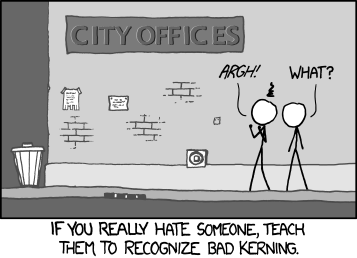
\includegraphics[scale=1,resolution=150]{graphics/kerning.png}
	\caption{``Kerning'' (\url{https://www.xkcd.com/1015}) by Randall Munroe is licensed under \mbox{CC~BY-NC~2.5}.}
	\label{fig:latex:unicode}
\end{figure}

%Another thing \LaTeX{} does is combine characters which look awkward together into one typographic entity called a \emph{ligature}. See \reffig{latex:ligature} for an example.

%\begin{figure}
%	\centering
%	{\Huge f{}i}~{\Huge fi}
%	\caption{Illustration of a ligature. In particular, the ``dots'' of the f and i are too close to look good (at least in normal text size) so instead they are made to coincide.}
%	\label{fig:latex:ligature}
%\end{figure}	

\subsection{Alignment and Hyphenation}
\index{justified}
\index{ragged}
\index{fully justified}
\index{full justification}
\index{left-aligned}
\index{right-aligned}
\index{centered}
In languages read left-to-right the left edge should normally be \emph{flushed} (aligned). Many WYSIWYG programs therefore defaults to \emph{left-aligned} where the right edge is \emph{ragged}. In \LaTeX{}, the default alignment is \emph{full justification} which means both edges are flushed (see \reffig{latex:alignment}). Both are commonly used. Advocates of left-aligned text argue that the ragged right edge helps the eye keep track of which line you're on, while justified text is considered more formal and many (including me) thinks it looks neater. Of course you have \emph{right-aligned} text and \emph{centered} text as well (which is ragged on both edges). In \LaTeX{} you can change the alignment either by putting the text in an environment or by using a switch. Both variants are found in \reftab{latex:alignment}.

\begin{table}
	\centering
	\caption{Alignment environments and switches}
	\begin{tabular}{lll}
	\hline
					& Environment			& Switch					\\
	\hline
	Left-aligned		& \latexin{flushleft}	& \latexin{\raggedright}	\\
	Right-aligned	& \latexin{flushright}	& \latexin{\raggedleft}	\\
	Centered			& \latexin{center}		& \latexin{\centering}
	\end{tabular}
	\label{tab:latex:alignment}
\end{table}

\index{tracking}
Full justification is achieved by stretching the spacing between characters (known as \emph{tracking}, not to be confused with kerning). To avoid the gaps getting unpleasantly large, \LaTeX{} often breaks up words with hyphens so they can be split across multiple lines. Normally you do not have to worry about this, but sometimes you may disagree with how \LaTeX{} splits words. In the preamble you can add hyphenation rules to a list of words like this:

\latexone{\hyphenation{tech-nol-o-gy cryp-tog-ra-phy}}
\noindent This allows the word ``technology'' and ``cryptography'' to be split everywhere you inserted a hyphen. You may be surprised by the amount of hyphens used in this example, but this is, in fact, how these words should hyphenated according to Merriam-Webster dictionary. People have many opinions about hyphenation rules, and you may of course choose to be more conservative than the Merriam-Webster dictionary, but try not to be too strict. You're not supposed to redefine every word you use.

\begin{figure}
	\centering\tiny\hfill%
	\begin{minipage}{0.4\textwidth}
		\raggedright
		Lorem ipsum dolor sit amet, consectetur adipiscing elit, sed do eiusmod tempor incididunt ut labore et dolore magna aliqua. Ut enim ad minim veniam, quis nostrud exercitation ullamco laboris nisi ut aliquip ex ea commodo consequat. Duis aute irure dolor in reprehenderit in voluptate velit esse cillum dolore eu fugiat nulla pariatur. Excepteur sint occaecat cupidatat non proident, sunt in culpa qui officia deserunt mollit anim id est laborum.
	\end{minipage}\hfill%
	\begin{minipage}{0.4\textwidth}
		Lorem ipsum dolor sit amet, consectetur adipiscing elit, sed do eiusmod tempor incididunt ut labore et dolore magna aliqua. Ut enim ad minim veniam, quis nostrud exercitation ullamco laboris nisi ut aliquip ex ea commodo consequat. Duis aute irure dolor in reprehenderit in voluptate velit esse cillum dolore eu fugiat nulla pariatur. Excepteur sint occaecat cupidatat non proident, sunt in culpa qui officia deserunt mollit anim id est laborum.
	\end{minipage}\hfill~
	\caption{Left-aligned vs. justified text}
	\label{fig:latex:alignment}
\end{figure}

\subsection{Line Lengths}
Some people think \LaTeX{} produces wastefully large margins, and tries to enforce smaller margins. However, typographists know that the mind gradually gets unfocused by the end of the line, and refocuses again for the next line. Too longs lines also makes it harder to jump to the start of the next line, while too short lines makes you switch line too often which disrupts reading. 

When \LaTeX{} has a margin of more than 4~cm on an A4 paper, it's just because of this. Books are often written in the slightly smaller format B5, while magazines and scientific journals often split the pages in two columns using the option \latexin{twocolumn}, e.g.:

\latexone|\usepackage[a4paper,twocolumn]{article}|
\noindent You may want to consider something like this before reducing margin size. If you \emph{still} have to reduce margin size, the package you need to look into is named \latexin{geometry}.

As we've seen, \LaTeX{} takes care of a whole deal for us, and if we decide to change some of \LaTeX{}'s default behavior we may want to ask why \LaTeX{} did it that way the first place? However, some formatting \LaTeX{} just can't do for us.

While there are plenty of studies on what makes text readable, not all of them agree and people have lots of different opinions. Using \LaTeX{}, you can be certain to make a document which is generally accepted as good typesetting.

\section{References}
\index{reference}
\index{\latexin{\label}}
\index{\latexin{\ref}}
Often, especially in documents of a professional nature, we'd like to refer to a previous (or future) chapter or section. Just writing ``Chapter~2'' in pure text works fine as long as you don't change anything, but as soon as you insert a chapter \emph{in front of} Chapter~2, such that Chapter~2 becomes Chapter~3, your reference becomes invalid. \LaTeX{} allows you to mark a chapter or section with a \emph{label} using the \latexin{\label} command, and then refer to it using the \latexin{\ref} command.

\index{non-break-space}
Consider the example in \reflst{latex:references}. Here we have labeled the introduction chapter with the label \latexin{ch:introduction} and the ``Scientific Instruments'' section with \latexin{sec:instruments} by using the \latexin{\label} command immediately after e.g.\ the \latexin{\chapter} command. The labels are not visible in the document, but we can now use \latexin{\ref} to get the number of that chapter or section. In this example, \latexin{\ref{sec:instruments}} would evaluate to ``2.1''. Since we don't want \LaTeX{} to break the line in the middle of ``Section~2.1'' we use a \emph{non-break-space}~(\latexin{~}) here.

\begin{listing}
	\begin{minted}[frame=lines,linenos]{latex}
		\chapter{Introduction}\label{ch:introduction}
		This paper is about\ldots

		\chapter{Method}
		The scientific method used is\ldots

		\section{Scientific Instruments}\label{sec:instruments}
		Below is a list of instruments used\ldots

		\chapter{Results}
		As described in Chapter~\ref{ch:introduction}\ldots

		\ldots possibly due to tolerance in the instruments
		described in Section~\ref{sec:instruments}.
	\end{minted}
	\caption{Example of using references}
	\label{lst:latex:references}
\end{listing}

In this example we have prefixed the label of the chapter by \latexin{ch:} and the label of the section by \latexin{sec:}. This is by no means necessary, \LaTeX{} do not care about what the label is as long as the reference matches the label. However, it is considered good practice to add such a prefix since it becomes clearer (in the code) what you're referring to. As we will see later, we can also references other kinds of contents which makes this point even more valid. \reftab{latex:label} shows suggested prefixes for different kinds of contents.

\begin{table}
	\centering
	\caption{Suggested label prefixes}
	\begin{tabular}{lll}
	\hline
	\latexin{ch:}	&	Chapters													\\
	\latexin{sec:}	&	Sections, subsections and subsubsections					\\
	\latexin{fig:}	&	Figures													\\
	\latexin{tab:}	&	Tables													\\
	\latexin{eq:}	&	Equations
	\end{tabular}
	\label{tab:latex:label}
\end{table}

Since \LaTeX{} writes a list of chapters and sections to an auxiliary file \emph{after} it has run through the .tex-files, changes of labels, or the order of labels, will only be effective after you've compiled the document twice. References to labels which doesn't exist in this auxiliary file yet is simply indicated by ``\textbf{??}'' in the PDF.

\section{New Commands}\label{sec:latex:newcommand}
\index{\latexin{\newcommand}}
\LaTeX{} allows you to define your own commands, and this is a suitable time to learn how. For instance, adding the following line somewhere in the preamble:

\latexone{\newcommand{\myname}{Peter}}
\noindent makes a new command \latexin{\myname} and every time you write \latexin{\myname} it is replaced by ``Peter''. Very nice if you plan to change your name in the foreseeable future!

A perhaps more useful example is to add the following custom commands to your preamble:

\begin{minted}[frame=none,numbers=none]{latex}
	\newcommand{\refch}[1]{Chapter~\ref{ch:#1}}
	\newcommand{\refsec}[1]{Section~\ref{sec:#1}}
	\newcommand{\reffig}[1]{Figure~\ref{fig:#1}}
	\newcommand{\reftab}[1]{Table~\ref{tab:#1}}
	\newcommand{\refeq}[1]{(\ref{eq:#1})}
\end{minted}
The option \latexin{[1]} means that the new command takes one argument, and the token \latexin{#1} is replaced by that (the first) argument. Then, writing \latexin{\refsec{instruments}} becomes equivalent to writing \latexin{Section~\ref{sec:instruments}} which evaluates to ``Section~2.1'' (in English, as opposed to some other languages, ``section'' is capitalized when talking about a particular section). Not only is it shorter and easier to write \latexin{\refsec{instruments}}, but it also becomes easier redefine your style later on. For instance, if you figure that you don't want to write ``Section'' but only its abbreviation ``Sec.'' you only have to change it one place. Notice that these commands expect you to follow the convention outlined in \reftab{latex:label}.

\subsection{Renew Commands}
\index{\latexin{\renewcommand}}
A command which is built-in to \LaTeX{} or that is already defined in a package can be redefined using the \latexin{\renewcommand}. It works in exactly the same way as \latexin{\newcommand}, and we have already used it in \refsec{latex:title}, which is a typical example. Whenever \LaTeX{} needed a date separator, it used the command \latexin{\dateseparator}, which we can redefine as we please.

\section{Figures}\label{sec:latex:figures}
\index{\latexin{\includegraphics}}
Graphics are included using the command \latexin{\includegraphics} provided by the \latexin{graphicx} package (remember to add this package to your preamble before making figures). However, there's usually more to a figure than just the graphics itself. This code can be used as a starting point when making a figure (actually, this is the exact code used to make \reffig{latex:texmaker}):

\begin{minted}{latex}
	\begin{figure}
		\centering
		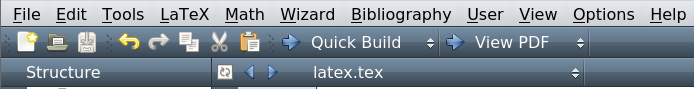
\includegraphics[width=\textwidth]{graphics/texmaker.png}
		\caption{Texmaker toolbar}
		\label{fig:texmaker}
	\end{figure}
\end{minted}

\index{float}
\index{\latexin{figure}}
First of all, everything related to the figure goes inside an environment called \latexin{figure}. I usually place this straight under the paragraph where I first made a reference to the figure. However, the \latexin{figure} environment is a \emph{float} which means that it will not appear where you put it, but as close as possible where \LaTeX{} finds a place which is typographically not too ugly. It kind of ``floats'' around. This feels very unnatural to many new users of \LaTeX{}, but try to get used to it. Only rarely do you have to force the placement of a float yourself (I've only done so once in this whole book). If you \emph{really} have to force the placement, you can add the ``here'' option to the figure environment by changing the first line to the following:

\latexone{\begin{figure}[h]}
\noindent You still are not guaranteed the figure will be exactly where you place it, but it usually gets closer.

\index{\latexin{\centering}}
The first thing inside the environment is the \latexin{\centering} switch which centers everything inside the \latexin{figure} environment (which is the scope of the switch), in particular the figure and its caption.

%The first command inside the environment is \latexin{\centering}. This is a switch which center-align the graphics and everything else inside the scope of the \latexin{figure} environment. And now we are ready to include the graphics using the \latexin{\includegraphics} command. As you can see, the author prefers to put all the graphics inside a separate subfolder called \verb|graphics|.

\index{\latexin{\textwidth}}
\index{\latexin{width}}
Then, the figure is included using \latexin{\includegraphics}. The author prefers to put all images inside a separate subfolder called \verb|graphics|. Next, the option \latexin{width=\textwidth} tells \LaTeX{} that the graphics should be as wide as the text on the page. The height scales accordingly. If you only want it to be e.g.\ 60\% as wide as the text you could change it to

\latexone{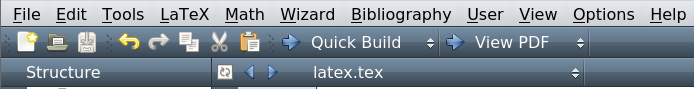
\includegraphics[width=0.6\textwidth]{graphics/texmaker.png}}
\noindent We'll look further into image size in a second.

\index{caption}
\index{\latexin{\caption}}
To give the figure a \emph{caption}, the text ``Figure 4.1: Texmaker toolbox'' which sits below the figure, we use the \latexin{\caption} command. We could also have placed \latexin{\caption} before \latexin{\includegraphics} to get the caption on top of the figure, however, captions typically appear at the bottom of floats. The enumeration appear automatically, just as for chapters.

At last, we have given the figure a label which allows us to refer to the figure using \latexin{\ref}:

\latexone{Please see Figure~\ref{fig:texmaker}.}
\noindent or the custom made \latexin{\reffig} defined in \refsec{latex:newcommand}:
\latexone{Please see \reffig{texmaker}.}

\subsection{Image Formats}
While not strictly speaking a part of \LaTeX{}, it's very useful to also get acquainted with some image formats so you can make qualified decisions when including graphics into your document, regardless of whether you're making it yourself or whether it's pre-made.

\index{BMP}
\paragraph{BMP}
One of the most basic image formats is BMP (bitmap, file extension .bmp). This is \emph{uncompressed} images where each pixel is stored by (typically) 24 bits, one pixel after the other. Because of this, for large images with many pixels, the files tend to get somewhat large. For example, a full HD image of resolution $1920\times 1080$ pixels becomes approximately 6~MB\footnote{$1920\times 1080=2\,073\,600$ pixels or 2~megapixels for short. Each pixel consumes 24 bits or 3 bytes since one byte equals 8 bits. Since each kilobyte is 1024 bytes and each megabyte is 1024 kilobytes we get $2\,073\,600\cdot 3/1024^2 \approx 6\,\mathrm{MB}$.}. Fortunately, it is possible to \emph{compress} images so they consume less space---often to less than a tenth, depending on the exact content of the image---and you are advised to always do so.

\index{JPEG}
\paragraph{JPEG} One compressed format which is suitable for photographs are JPEG (Joint Photographic Experts Group, file extension .jpg or .jpeg). It greatly compresses image files at the cost of image quality. The trade-off between size and quality is determined by a \emph{quality factor} which is a number which can be adjusted in the range 0--100. Higher means better quality.

\index{PNG}
\paragraph{PNG} However, JPEG is not well suited for graphics with simpler geometry, fewer colors and abrupt edges (for instance letters), as it tends to ``smear'' out the abrupt edges across small blocks. Especially around text. For such graphics, PNG (Portable Network Graphics, file extension .png) is recommended. Contrary to JPEG, PNG is a \emph{lossless} format which means the the compression do \emph{not} compromise the quality (no losses). The file size just gets smaller! The compression level for PNG can be adjusted from 1--9. Higher means better compression at the cost of (insignificantly) slower processing. The downside is that PNG is not able to compress photos as much as JPEG, although it often compress simpler graphics files more. The compression achieved depends on the contents on the image.

\begin{figure}
	\centering
	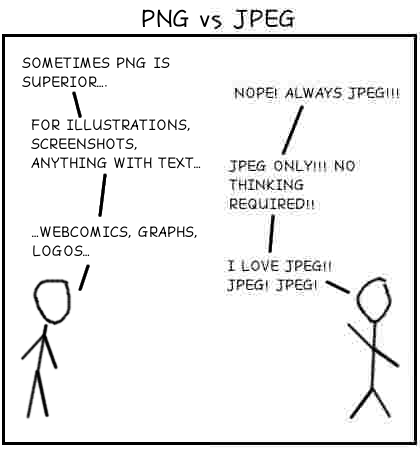
\includegraphics[scale=1,resolution=150]{graphics/jpg_vs_png.png}
	\caption{PNG vs.\ JPEG. The right half is compressed with excessively low quality JPEG while the left is PNG. Courtesy of Louis Brandy, \url{http://lbrandy.com}.}
	\label{fig:latex:pngjpeg}
\end{figure}

\index{Gimp}
An excellent tool for editing images of these formats is \emph{Gimp}, which is a free alternative to PhotoShop. Gimp has plenty of tutorials online and will not be covered here.

\index{PPI}
\index{pixels per inch}
\index{dots per inch}
How many pixels an image consists of does not really say anything about its physical size on print. Because how large is a pixel? How densely are they packed? For a computer monitor, there's typically about 100--150 \emph{pixels per inch} (PPI). To get a sufficiently smooth picture on print, however, you should have at least 300~PPI. Then, how many pixels do you need to make a nice figure of $5\times 2\,\mathrm{cm}$? The answer can be calculated as follows:

\begin{align}
	\text{Width:}\quad	&	\frac{5}{2.54}\,\mathrm{in}\cdot 300\,\mathrm{PPI}=591\,\mathrm{px}	\\
	\text{Height:}\quad	&	\frac{2}{2.54}\,\mathrm{in}\cdot 300\,\mathrm{PPI}=236\,\mathrm{px}
\end{align}
The number 2.54 is merely a conversion factor from centimeters to inches.

Once you've made an image of this many pixels, you can include it in your document with this command to get the right size and 300~PPI

\latexone{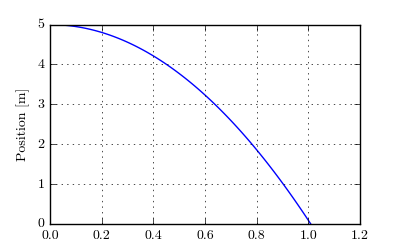
\includegraphics[width=5cm]{graphics/figure.png}}
\noindent However, many image editing programs, Gimp included, allows you to specify the number of PPI when creating a new image. This is embedded directly into the image for \LaTeX{} to find it. Then it is much simpler to choose an image size of $5\si{cm}\times 2\si{cm}$ and 300~PPI in the image editing program and insert it by

\index{\latexin{scale}}
\latexone{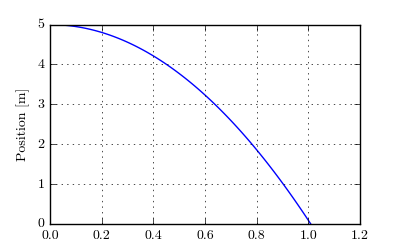
\includegraphics[scale=1]{graphics/figure.png}}
\noindent The \latexin{scale} option here tells it to print it in full size, and since \LaTeX{} knows both the number of pixels and PPI it can figure out the size. Strictly speaking, you could get away with a picture of 100~PPI if you put \latexin{scale=0.33}, since effectively, you still have 300~PPI on print (or 300 \emph{dots per inch} which is the correct term once you get it on paper).

%\begin{figure}
%	\centering
%	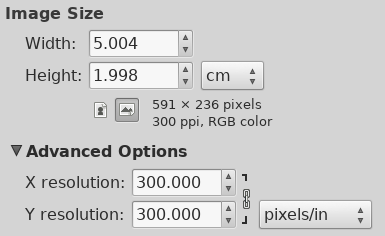
\includegraphics[resolution=150,scale=1]{graphics/gimp.png}
%	\caption{An excerpt from the Gimp ``Create a New Image'' dialog.}
%	\label{fig:latex:gimp}
%\end{figure}

Often you can get away not bothering about any of this. You create an image, specifying the widht of the image in terms of \latexin{\textwidth} and it turns out good. But if your image ever looks poor, maybe you've used too few PPI. And if you make a figure with text labels on it, you often end up unintentionally scaling the text to look very small or big. Not to speak of the annoyance of having text not the same size as in the rest of the document!

\index{point (pt)}
The remedy when using text in images, is to use a font size of 10~pt in the image, at least 300~PPI, and include it using \latexin{scale=1}. A typographic point (pt), by the way, is 1/72 of an inch. To achieve the best effect, you could also download the Computer Modern typeface to get the same font in the figures. Computer Modern con be downloaded here:

~\\
\urlone{http://www.ctan.org/tex-archive/fonts/cm/ps-type1/bakoma/otf}

The file \verb|cmr10.otf|, for instance, is the Computer Modern Roman font in 10~pt size. Most operating systems will offer to install it if you open it, and subsequently, you can find it as cmr10 in all your programs.

\index{SVG}
\index{raster graphics}
\index{vector graphics}
\paragraph{SVG} All the image formats covered so far are \emph{raster graphics}, that is, a rectangular grid of square pixels of different colors. On the other hand, \emph{vector graphics} do not consist of pixels at all but rather of a description of geometric shapes. It may for instance specify ``draw a triangle between the three vertices with the following coordinates\ldots'', or ``draw a curve between these points'', and so on. This has the advantage that as you zoom in, the image does not get pixelated. See \reffig{latex:arrow}. A common format for vector graphics is SVG (Scalable Vector Graphics, file extension .svg).

%This is very advantageous as it means you can just create the graphics first, and then tweak the size relative to the \latexin{\textwidth} after you've included it in your document without having to worry that you get too poor resolution.
Again, if you use text labels in the figure, use 10~pt sized cmr10 font and include it using \latexin{scale=1}. If your figure does not contain text, you have the advantage that since vector graphics scales perfectly, you can choose the size using e.g. \latexin{text=0.7\textwidth} after you've made it.
% If you include text labels in your vector graphics, however, you want to make sure it is 10~pt (same as in \LaTeX{}) and use \latexin{scale=1}.


\begin{figure}
	\centering
	\begin{minipage}[b]{0.32\linewidth}
		\centering
		
\includegraphics[scale=1]{graphics/arrow.pdf}
		\subcaption{Original size}
	\end{minipage}%
	\begin{minipage}[b]{0.32\linewidth}
		\centering
		
\includegraphics[scale=10]{graphics/arrowCut.pdf}	
		\subcaption{Vector graphics}
	\end{minipage}%
	\begin{minipage}[b]{0.32\linewidth}
		\centering
		
\includegraphics[scale=10]{graphics/arrowCut.png}	
		\subcaption{300~PPI Raster graphics}
	\end{minipage}%	
	\caption{Scaling vector graphics vs.\ raster graphics to 1000\%.}
	\label{fig:latex:arrow}	
\end{figure}

\index{InkScape}
While vector graphics is perfect whenever you can use it (illustrations, graphs, etc.), unfortunately you cannot reduce a photo to mere geometric objects and store them in a vector graphics file format. You also cannot take an illustration which is already made in raster graphics and magically turn the pixels into geometric objects. Instead, you have to make the illustrations by creating geometric objects from the very beginning. A highly recommended program to do this is InkScape. Fortunately, it's also much easier to use than for instance Gimp or PhotoShop. You may even get started simply by clicking and trying.

\index{PDF}
\paragraph{PDF} Unfortunately, \LaTeX{} do not support the SVG format. Instead, you must save it to a PDF containing only the image. However, if you use InkScape, it is advised to keep a copy of the image in InkScape SVG format since it allows you to edit the image by means of the same geometric objects later on. 

\index{EPS}
\paragraph{EPS} Maybe you remember we mentioned that some compile their documents using \verb|latex| rather than \verb|pdflatex|? Well, if so, they cannot use any of the formats mentioned so far but have to convert all images to EPS (Encapsulated PostScript). We'll stick to \verb|pdflatex| and not bother about this format, but if you ever stumble upon a .tex-file with EPS images included you know they compiled it using \verb|latex|.

To summarize, you are advised you to use PDF vector graphics whenever you can (figures, graphs, illustrations, etc.) and JPEG for photos. If you happen to have an illustration which is already in a raster format you should use PNG. It is a good habit to always trim white edges surrounding the images in whichever tool you use. See \refsec{bash:imagemagick} for how to do this to multiple images at once. See also \refsec{python:plotting} for how to make graphs using Python.

\begin{figure}
	\centering
	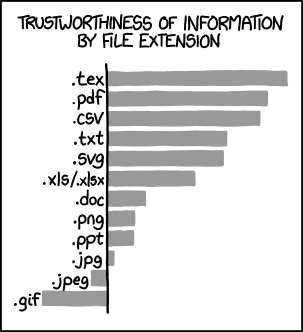
\includegraphics[scale=0.48,resolution=72]{graphics/file_extensions.png}
	\caption{``File Extensions'' (\url{https://xkcd.com/1301}) by Randall Munroe is licensed under \mbox{CC~BY-NC~2.5}.}
	\label{fig:latex:unicode}
\end{figure}

Finally, the knowledge acquired in this section is applicable outside of typesetting as well, for instance to web design. You may have different priorities there, e.g.\ higher quality on print, smaller files on the web, but the formats and their advantages/disadvantages are all the same.

\section{Exercises}
\begin{ExerciseList}
	\Exercise Create an A4 \latexin{article} containing paragraphs 1--5 of Lorem Ipsum in an unnumbered section named ``Lorem Ipsum''. Unnumbered sections are written using \latexin{\section*} rather than \latexin{\section}.
	\Answer ~\\ \inputminted[frame=lines]{latex}{latex/exer_lipsum.tex}
	
	\Exercise Change document layout to use two columns.
	\Answer Replace
	\latexone{\documentclass[a4paper]{article}}
	with
	\latexone{\documentclass[a4paper,twocolumn]{article}}
	
	\Exercise Try out left-alignment.
	\Answer Replace
	\begin{minted}{latex}
		\lipsum[1-5]
	\end{minted}
	with
	\begin{minted}{latex}
		\raggedright
		\lipsum[1-5]
	\end{minted}
	or
	\begin{minted}{latex}
		\begin{flushleft}
			\lipsum[1-5]
		\end{flushleft}
	\end{minted}

	\Exercise Create an image \verb|fig1.png| of $7\times 4\,\mathrm{cm}$ at 300~PPI. If you use Gimp you can select these parameters when you choose File$\rightarrow$New. Draw some contents (exactly what is not important) and add some text using a serif font (preferrably cmr10) at 10~pt. Make sure that the contents only consume a small part of the image. Insert it as a figure to a document using \latexin{scale=1}. Is the text the same size as the text in the document?
	\Answer Yes, it should be. If you used a different font there may be a small discrepancy.	
	
	\Exercise Now adjust the image to 72~PPI (which is default in many programs) and store as \verb|fig2.png|, but keep the physical size (at least as closely as possible). This can be done in Gimp by entering Image$\rightarrow$Scale~Image. Insert it in the document. How does this affect the quality and size?
	\Answer The size should remain, but the quality is seriously degraded. Had you scaled the image down by a factor 72/300=0.24 you would have kept the quality.
	\Exercise Trim away the white edges of \verb|fig1.png| and re-compile. In Gimp: Image$\rightarrow$Autocrop~Image.	
	\Exercise Create a small vector image \verb|fig3.pdf|. Insert some text using a serif font (preferably cmr10) at 10~pt and perhaps some lines or circles. If you use InkScape, white edges can be trimmed away using File$\rightarrow$Document~Properties$\rightarrow$Resize~page~to~content before saving the image. Insert to \LaTeX{} document. Is the text the right size?
	\Answer Yes, it should be. If you used a different font there may be a small discrepancy.	
	
	\Exercise Open the document containing both \verb|fig1.png| and \verb|fig3.pdf| and zoom in. Do you notice the difference?
	\Answer Only the raster graphics should get pixelated.
	
	\Exercise If you've read \refsec{python:plotting}, insert a plot into the document.
	\Exercise Add labels to a couple of the figures and sections and try to write some dummy text where you refer to them using \latexin{\ref}.
	\Exercise Add the custom reference commands from \refsec{latex:newcommand} to your preamble and replace the usage of \latexin{\ref} by those.
\end{ExerciseList}

\section{Tables}
Tables are in many ways similar to figures. Let's see how to make \reftab{latex:distance}:

\begin{minted}{latex}
	\begin{table}
		\centering
		\caption{Distance between cities in km}
		\begin{tabular}{l|ccc}
			            & Oslo   & Trondheim & Bergen \\
			\hline
			Oslo        & 0      & 494       & 463    \\
			Trondheim   & 494    & 0         & 699    \\
			Bergen      & 463    & 699       & 0
		\end{tabular}
		\label{tab:distance}
	\end{table}
\end{minted}

\begin{table}
	\centering
	\caption{Distance between cities in km}
	\begin{tabular}{l|ccc}
					& Oslo	& Trondheim	& Bergen		\\
		\hline
		Oslo			& 0		& 494		& 463		\\
		Trondheim	& 494	& 0			& 699		\\
		Bergen		& 463	& 699		& 0
	\end{tabular}
	\label{tab:latex:distance}
\end{table}

The \latexin{table} environment is a float quite similar to \latexin{figure} and many of the commands inside it are also familiar from when we discussed figures (\refsec{latex:figures}). As for \latexin{figure}, you can use the \latexin{h} option to get the table closer to where you place it in the code. A minor detail, is that the caption is on top. Some authors strictly obey the rule that floats always have captions on bottom, while others use captions on bottom for figures, captions on top for tables.

Anyhow, the only new thing inside \latexin{table} is the \latexin{tabular} environment. The \latexin{tabular} environment has one mandatory argument (here set to \latexin{l|ccc}) which specifies the number of columns, and their formatting. The letters \latexin{l}, \latexin{c} and \latexin{r} represents a column which is left, center or right-aligned, respectively. In our example we have one left-aligned column and three centered columns. In addition, you may separate columns by single or double borders by putting \latexin{|} or \latexin{||} between their letters. \emph{Inside} the \latexin{tabular} environment, cells are separated by \latexin{&} while rows are separated by \latexin{\\}. One or two \latexin{\hline} commands may be used to separate rows by single or double borders.

\subsection{Spanning Multiple Columns}
Sometimes we want a cell to span several columns, like the cell that says ``Speed'' in \reftab{latex:speed}. This is done by a command named \latexin{\multicolumn} which takes three arguments. The first is the number of columns to span across, the second is the alignment, and the third is the contents of the cell. The code for the whole \latexin{tabular} environment is shown here:

\begin{table}
	\centering
	\caption{Speed of animals (source: \url{speedofanimals.com})}
	\begin{tabular}{|l|c|c|}
		\hline
					& \multicolumn{2}{c|}{Speed}		\\
		\cline{2-3}
					& km/h		& mph				\\
		\hline
		Elk			& 72.4		& 45.0				\\
		Cat			& 48.0		& 29.8				\\
		Pig			& 17.7		& 11.0				\\
		\hline
	\end{tabular}
	\label{tab:latex:speed}
\end{table}

\begin{minted}{latex}
		\begin{tabular}{|l|c|c|}
			\hline
					   & \multicolumn{2}{c|}{Speed}	\\
			\cline{2-3}
					   & km/h	& mph				 \\
			\hline
			Elk		& 72.4	& 45.0				\\
			Cat		& 48.0	& 29.8				\\
			Pig		& 17.7	& 11.0				\\
			\hline
		\end{tabular}
\end{minted}

Notice that we use \latexin{\multicolumn} in the first cell we wanted to span over, and simply skip the subsequent ones. Moreover, the alignment in \latexin{\multicolumn} is \latexin{c|} rather than \latexin{|c|}. That's because a border is drawn already when \LaTeX{} hits \latexin{&}. Having \latexin{|c|} would produce two borders on top of one another which may be slightly visible. My advise is to start without borders in the spanned cell and add one by one while you inspect the results.

We have also introduced a new command \latexin{\cline{2-3}} which indicates that a border should be drawn but only between rows 2--3.

\subsection{Spanning Multiple Rows}
To span multiple rows you must first include the package \latexin{multirows}, then you use the command \latexin{\multirows} in the first cell you want to span over, and let the next ones be empty. \reftab{latex:languages} is generated using the following tabular:

\begin{table}
	\centering
	\caption{Programming languages}
	\begin{tabular}{|ll|}
		\hline
		\multirow{3}{*}{Interpreted}		& Python		\\
										& Lisp		\\
										& JavaScript	\\
		\hline
		\hline
		\multirow{4}{*}{Compiled}		& C++		\\
										& Java		\\
										& Haskell	\\
										& Pascal		\\
		\hline
	\end{tabular}
	\label{tab:latex:languages}
\end{table}

\begin{minted}{latex}
\begin{table}

	\begin{tabular}{|ll|}
		\hline
		\multirow{3}{*}{Interpreted} & Python     \\
		                             & Lisp       \\
		                             & JavaScript \\
		\hline
		\hline
		\multirow{4}{*}{Compiled}    & C++        \\
		                             & Java       \\
		                             & Haskell    \\
		                             & Pascal     \\
		\hline
	\end{tabular}
\end{table}
\end{minted}

The first argument of \latexin{\multirow} is the number of rows to span across, the second argument is the width of the cell, while the last is the contents. The width is usually auto-adjusted by using \latexin{*}.

Many people find writing tables in \LaTeX{} cumbersome, and consequentially, some tools has been made to write the code for you. Perhaps the most readily available if you use Texmaker is the built-in wizard found in the menu Wizard$\rightarrow$Quick~Tabular. Alternatively, if you prefer to write tables in a full-blown spreadsheet program like Microsoft Excel with all its features you can download the macro Excel2LaTeX here:

~\\
\url{http://www.ctan.org/tex-archive/support/excel2latex} \\

\noindent For OpenOffice Calc there's an equivalent named Calc2LaTeX which you can find here:

~\\
\url{http://calc2latex.sourceforge.net} \\

\noindent This one also works for LibreOffice Calc. Their installation and use is described on the mentioned pages.

\section{Lists}
List are written by enclosing a bunch of items in an environment which says what kind of list it is. For instance, an \latexin{itemize} environment is used to make a list of bullet points whereas \latexin{enumerate} is used to make an enumerated list. \reflst{latex:lists} illustrates how to make various kinds of lists.

\begin{listing}
	\rule{\textwidth}{0.4pt}
	\begin{minipage}[t]{0.49\textwidth}
		\begin{minted}{latex}
			\begin{itemize}
			  \item Coffee
			  \item Milk
			  \item Butter
			\end{itemize}

			\begin{enumerate}
			  \item Wash clothes
			  \item Tumble dry
			  \item Iron
			\end{enumerate}		

			\begin{description}
			  \item[Python] An interpreted
			  multi-paradigm programming
			  language
			  \item[C] A compiled procedural
			  programming language
			  \item[Java] A compiled object-
			  oriented programming language
			\end{description}	
		\end{minted}
	\end{minipage}\hfill\vline\hfill
	\begin{minipage}[t]{0.49\textwidth}
			\begin{itemize}
			  \item Coffee
			  \item Milk
			  \item Butter
			\end{itemize}
			\vspace{0.6em}
			\begin{enumerate}
			  \item Wash clothes
			  \item Tumble dry
			  \item Iron
			\end{enumerate}		
			\vspace{0.6em}
			\begin{description}
			  \item[Python] An interpreted
			  multi-paradigm programming
			  language
			  \item[C] A compiled procedural
			  programming language
			  \item[Java] A compiled object-%
			  oriented programming language
			\end{description}				
	\end{minipage}\\[0.5em]
	\rule{\textwidth}{0.4pt}
	\caption{Different kinds of lists}
	\label{lst:latex:lists}
\end{listing}

Lists may also be nested as illustrated in \reflst{latex:nestedlists}. You may notice that every time we enter an environment we choose to indent the lines one tab further (except for the \latexin{document} environment). This is not necessary, but makes the code cleaner to read.

\begin{listing}
	\rule{\textwidth}{0.4pt}
	\begin{minipage}[t]{0.49\textwidth}
		\begin{minted}{latex}
			Master plan:
			\begin{enumerate}
				\item Buy farm
				\item Buy animals
				\begin{enumerate}
					\item Cows
					\item Sheep
					\item Chickens
				\end{enumerate}
				\item Start farming
			\end{enumerate}	
		\end{minted}
	\end{minipage}\hfill\vline\hfill
	\begin{minipage}[t]{0.49\textwidth}
			Master plan:
			\begin{enumerate}
				\item Buy farm
				\item Buy animals
				\begin{enumerate}
					\item Cows
					\item Sheep
					\item Chickens
				\end{enumerate}
				\item Start farming
			\end{enumerate}							
	\end{minipage}\\[0.5em]
	\rule{\textwidth}{0.4pt}
	\caption{Nested lists}
	\label{lst:latex:nestedlists}
\end{listing}

\section{Equations}\label{sec:latex:equations}

\subsection{Math Mode}
\index{math mode}
One of \LaTeX{}'s main strength is typesetting equations. Just imagine trying to writing something like this (the Fourier transform) in a WYSIWYG tool:

\begin{equation}
	\hat{f}(\omega)=\frac{1}{\sqrt{2\pi}}
	\int\limits_{-\infty}^\infty f(t)e^{i\omega t} \,\mathrm{d}t
	\label{eq:latex:fourier}
\end{equation}
\noindent Using \LaTeX{} this is no problem. Let's start just a bit simpler, though, with Ohm's law:

\index{\latexin{equation}}
\begin{minted}[frame=none]{latex}
	\begin{equation}
		U = R \cdot I		
	\end{equation}
\end{minted}
which becomes:

\begin{equation}
	U = R \cdot I
	\label{eq:latex:ohm}
\end{equation}

Inside the \latexin{equation} environment you're in so-called \emph{math mode}, where a special syntax is used to write equations. \latexin{\cdot}, for instance, represents the multiplication symbol. Many of the equations we write require the package \latexin{amsmath} as well as symbols from \latexin{amssymb}. 

Equations are automatically enumerated, and as you might have guessed, you can use references as well. For instance, you can add a label to the above code:
\begin{minted}[frame=none]{latex}
	\begin{equation}
		U = R \cdot I
		\label{eq:ohm}		
	\end{equation}
\end{minted}
and then refer to it as follows:

\latexone{Ohm's law is given in (\ref{eq:ohm}).}
\noindent or equivalently, using the custom \latexin{\refeq} command defined in \refsec{latex:newcommand}:
\latexone{Ohm's law is given in \refeq{ohm}.}
\noindent which evaluates to:

\begin{quote}
	Ohm's law is given in \refeq{latex:ohm}.
\end{quote}

\index{\latexin{equation*}}
If an equation is rather unimportant, you may not even want to enumerate it, in which case you can use the \latexin{equation*} environment (starred version) in place of the usual \latexin{equation} environment.

\index{inline math mode}
You may also write math inside normal text. This is done using \emph{inline math mode} which is encapsulated using \latexin{$}\ignore{$}, like this:

\latexone{It turned out that $x=3.5$ was the correct answer.}
\noindent which becomes:

\begin{quote}
	It turned out that $x=3.5$ was the correct answer.
\end{quote}

\subsection{Units}
\index{variable}
\index{value}
In the inline equation in the above example, $x$ is the \emph{variable} and 3.5 is its numerical value. Variables are typeset in italic whereas numbers are in roman (upright). This happens automatically. However, if you want to add a \emph{unit}, say meters, the proper way to display it would be:

\begin{equation*}
	x = 3.5 \, \mathrm{m}
\end{equation*}
Thus the unit is in roman as opposed to the variable. This is achieved by writing (in math mode):

% Should actually be in math mode, e.g. encapsulated by $, to get right highlighting.
\latexone{x = 3.5 \, \mathrm{m}}

\latexin{\mathrm} is the math mode equivalent of \latexin{\textrm} from \reftab{latex:formatting}. It is often the case that a command which somehow alters the formatting has a differently named equivalent in math mode. Next, \latexin{\,} is used to insert a small space in front of the unit (you cannot just insert another space in the code, \LaTeX{} won't care). The following properly typeset expression demonstrates the aesthetics of having an extra space between number and unit, but not between number and variable:

\begin{equation*}
	2x = 7\,\mathrm{m}
\end{equation*}
If you have many expressions with units, however, you may want to familiarize yourself with the \latexin{siunitx} package (not covered here).

\subsection{More Equations}
Perhaps the easiest way to learn to typeset a wider range of equations is by example, so here we go. Superscripts and subscripts:

\newcommand{\eqlatexminwdith}{7cm}

\renewcommand{\arraystretch}{1.5}
\begin{tabular}{m{\eqlatexminwdith}l}
	\latexmin{x_i}			&	$x_i$			\\
	\latexmin{x^n}			&	$x^n$			\\
	\latexmin{x_i^n}			&	$x_i^n$			\\
	\latexmin{c_{ij}=a_ib_j}	&	$c_{ij}=a_ib_j$
\end{tabular}
\renewcommand{\arraystretch}{1}

\noindent Notice that we had to group together $ij$ on the left hand side. On the right hand side, $b$ is \emph{not} a subscript since \latexin{_} only applies to the first symbol unless a group is used. Normally, when subscripts and superscripts act like indices and exponents and such, they appear in italic. However, words and abbreviations (text) which occur inside equations should be typeset in roman, either by the use of \latexmin{\mathrm} or better, \latexmin{\text}. E.g. to denote the mass of the Sun one could write

\renewcommand{\arraystretch}{1.5}
\begin{tabular}{m{\eqlatexminwdith}l}
	\latexmin{m_{\text{sun}}}			&	$m_{\text{sun}}$
\end{tabular}
\renewcommand{\arraystretch}{1}

\noindent Sometimes, words or abbreviations are also used for variable names, such as $\text{GNP}$ for \emph{Gross National Product}. This is considered text too:

\renewcommand{\arraystretch}{1.5}
\begin{tabular}{m{\eqlatexminwdith}l}
	\latexmin{\text{GNP}=\ldots}			&	$\text{GNP}=\ldots$
\end{tabular}
\renewcommand{\arraystretch}{1}

Fractions and square roots:

\renewcommand{\arraystretch}{2.2}
\begin{tabular}{m{\eqlatexminwdith}l}
	\latexmin{3/4}				&	$\displaystyle 3/4$					\\
	\latexmin{\frac{3}{4}}		&	$\displaystyle \frac{3}{4}$			\\
	\latexmin{\frac{a+b}{2}}		&	$\displaystyle \frac{a+b}{2}$			\\
	\latexmin{\sqrt{n+\sqrt{n}}}	&	$\displaystyle \sqrt{n+\sqrt{n}}$		\\
\end{tabular}
\renewcommand{\arraystretch}{1}

\noindent Equations are often displayed slightly different depending on whether its inlined or not. \latexmin{\frac{3}{4}}, for instance becomes smaller: $\frac{3}{4}$. The square root symbol's size automatically adjusts to its contents. Parentheses and brackets, by default, do not. However, by using \latexin{\left} and \latexin{\right}, it does:

\renewcommand{\arraystretch}{2.2}
\begin{tabular}{m{\eqlatexminwdith}l}
	\latexmin{(3+2)}						&	$(3+2)$									\\
	\latexmin{(\frac{3}{4})}				&	$\displaystyle (\frac{3}{4})$	 (wrong)		\\
	\latexmin{\left(\frac{3}{4}\right)}	&	$\displaystyle \left(\frac{3}{4}\right)$	\\
	\latexmin{\left[\frac{3}{4}\right]}	&	$\displaystyle \left[\frac{3}{4}\right]$
\end{tabular}
\renewcommand{\arraystretch}{1}

Vectors:

\renewcommand{\arraystretch}{1.5}
\begin{tabular}{m{\eqlatexminwdith}l}
	\latexmin{\vec{v}}					&	$\displaystyle \vec{v}$ (default) or $\displaystyle \mathbf{v}$
\end{tabular}
\renewcommand{\arraystretch}{1}

\noindent Both styles for vectors are used a lot in the scientific literature, although the bold font is perhaps somewhat more common. To display vectors using bold font, the \latexin{\vec} command must be redefined in the preamble:

\latexone{\renewcommand{\vec}{\mathbf}}

Next, some mathematical functions and greek letters. First of all, it is incorrect to write:

\renewcommand{\arraystretch}{1.5}
\begin{tabular}{m{\eqlatexminwdith}l}
	\latexmin{sin\theta}					&	$\displaystyle sin\theta$ (wrong)
\end{tabular}
\renewcommand{\arraystretch}{1}

\noindent Functions such as $\sin$ have their own command, e.g.\ \latexmin{\sin}:

\renewcommand{\arraystretch}{1.5}
\begin{tabular}{m{\eqlatexminwdith}l}
	\latexmin{\sin\theta}					&	$\displaystyle \sin\theta$ 			\\
	\latexmin{\cos(\omega t)}				&	$\displaystyle \cos(\omega t)$ 		\\
	\latexmin{\tan(2\pi f)}					&	$\displaystyle \tan(2\pi f)$ 			\\
	\latexmin{\arctan 30\degree}				&	$\displaystyle \arctan 30\degree$		\\
	\latexmin{\log(10^x)}					&	$\displaystyle \log(10^x)$			\\
	\latexmin{\ln(e^x)}						&	$\displaystyle \ln(e^x)$
\end{tabular}
\renewcommand{\arraystretch}{1}

\noindent Mind that \latexin{\degree} is provided by the package \latexin{gensymb}.

You can see that such \emph{operator names} are in roman and that the spacing around them is slightly different. Often you can successfully guess the command for greek letters and operator names.  However, you may also need some operator name which simply is not predefined in \LaTeX:

\renewcommand{\arraystretch}{1.5}
\begin{tabular}{m{7cm}l}
	\latexmin{\operatorname{lb}(2^x)}						&	$\displaystyle \operatorname{lb}(2^x)$
\end{tabular}
\renewcommand{\arraystretch}{1}

Derivatives of various kinds are written as follows:

\renewcommand{\arraystretch}{2.2}
\begin{tabular}{m{7cm}l}
	\latexmin{f'(x)}										&	$\displaystyle f'(x)$								\\
	\latexmin{\dot{r}(t)}								&	$\displaystyle \dot{r}(t)$							\\	
	\latexmin{\frac{\mathrm{d}f}{\mathrm{d}x}}			&	$\displaystyle \frac{\mathrm{d} f}{\mathrm{d} x}$		\\
	\latexmin{\frac{\partial f}{\partial x}}				&	$\displaystyle \frac{\partial f}{\partial x}$
\end{tabular}
\renewcommand{\arraystretch}{1}

\noindent Often the $\mathrm{d}$ in differentials such as $\mathrm{d}x$ are written in roman, although not everyone adhere to this convention. The author finds it aesthetic and chooses to do so by using \latexmin{\mathrm}.

Integrals can be written with the limits either on top/bottom or to the right of the integral symbol depending on whether or not you use \latexmin{\limits}:

\renewcommand{\arraystretch}{2.5}
\begin{tabular}{m{7cm}l}
	\latexmin{\int_a^b f(x) \, \mathrm{d}x}			&	$\displaystyle \int_a^b f(x) \, \mathrm{d}x$			\\
	\latexmin{\int\limits_a^b f(x) \, \mathrm{d}x}	&	$\displaystyle \int\limits_a^b f(x) \, \mathrm{d}x$
\end{tabular}
\renewcommand{\arraystretch}{1}

\noindent The author suggests using the top/bottom notation normally, but not for inline as that ruins line spacing. It's customary to add some extra space (\latexmin{\,}) in front of the differential.

Admittedly, we have been picky in this section. Many authors, even of scientific publications, are sloppy or even unaware of when to use roman text, where to add additional spaces, and so forth. And usually no one cares.

\subsection{Align Equations}
Another math mode environment which may be of interest is the \latexin{align} environment. It allows you to line up several rows of equations, e.g.

\begin{minted}{latex}
	\begin{align}
		x   &= (a+b)(c+d)           \nonumber \\
			&= a(c+d)+b(c+d)		\nonumber \\
			&= ac+ad+bc+bd		  \label{eq:expansion}
	\end{align}
\end{minted}
to produce

\begin{align}
	x   &= (a+b)(c+d)		\nonumber \\
		&= a(c+d)+b(c+d)		\nonumber \\
		&= ac+ad+bc+bd
\end{align}
It resembles the \latexin{tabular} environment in that \latexin{&} separates ``cells'' and \latexin{\\} separates rows. The leftmost column is right-aligned while the second is left-aligned. Here, the equality signs line up. If more than two columns are used, they keep alternating between right and left-aligned.

\latexin{\nonumber} is used to turn off enumeration for a row. In this case it's actually just one equation split across multiple lines, so we only want one number. One could also line up distinct equations under one another, and give them separate labels, keeping one \latexin{\label} command per row.

\section{Exercises}
\begin{ExerciseList}
	\Exercise Typeset $v=s/t$ inline.
	\Answer ~\\ \latexone{$v=s/t$}
	
	\Exercise Typeset
		\begin{equation}
			v=\frac{s}{t}
		\end{equation}
	\Answer ~\\
	\begin{minted}{latex}
		\begin{equation}
			v=\frac{s}{t}
		\end{equation}
	\end{minted}

	\Exercise Typeset $v_0 = 7.2 \, \mathrm{m/s}$ inline.
	\Answer ~\\ \latexone{$v_0 = 7.2 \, \mathrm{m/s}$}
	
	\Exercise Typeset $\int_a^b f(t) \, \mathrm{d}t$ inline.
	\Answer ~\\ \latexone{$\int_a^b f(t) \, \mathrm{d}t$}
	
	\Exercise Typeset \refeq{latex:fourier}. Hint: Check out \latexin{\hat} and \latexin{\infty}.
	\Answer ~\\
	\begin{minted}{latex}
		\begin{equation}
			\hat{f}(\omega) = \frac{1}{\sqrt{2\pi}}
			\int\limits_{-\infty}^\infty f(t)e^{i\omega t} \,\mathrm{d}t
		\end{equation}
	\end{minted}	
	
	\Exercise Typeset the equation for the root mean square of $N$ data points:
		\begin{equation}
			x_\text{rms} = \sqrt{ \frac{1}{N} \sum_{i=1}^N x_i^2 }
		\end{equation}
		Hint: Check out \latexin{\sum}.
	\Answer ~\\
	\begin{minted}{latex}
		\begin{equation}
			x_\text{rms} = \sqrt{ \frac{1}{N} \sum_{i=1}^N x_i^2 }
		\end{equation}
	\end{minted}
	
\end{ExerciseList}

\section{Bibliography}
The standard tool to make a bibliography (list of references) in \LaTeX{} is \bibtex{}. \bibtex{} is a whole new universe with its own syntax and features, but we will limit ourselves to the most important parts.

\subsection{Database}
To use \bibtex{} you create a database of references in one or more separate .bib-files, and then you can cite those references anywhere in your text. An example .bib-file with three entries is shown in \reflst{latex:bibtex}. Each entry consists of a \emph{specification} of what type of reference it is, a \emph{key}, and a list of fields (\emph{parameter}--\emph{value} pairs). In \reflst{latex:bibtex} the we have three references, a book, an article from a scientific journal, and a website. Since citation of websites is a rather new phenomena there's no standardized way of doing it. We have used the catch-all specification \latexin{@misc} (miscellaneous).

\begin{listing}
	\inputminted[frame=lines,linenos]{latex}{latex/main.bib}
	\caption{A \bibtex{} file}
	\label{lst:latex:bibtex}
\end{listing}

The key is the first thing that follows inside the curly braces, and it's similar to labels of figures and tables; you use it when you want to cite the reference. It can be anything, but it's a good idea to always follow some sort of rule for how to write it. Here the key is the surname of the first author in lowercase followed by the year of publication.

Next, all the fields are separated by commas. The values are enclosed in either curly braces or quotation marks. With every type of specification some fields are mandatory. For an article for instance, you need its author, title, year of publication and which journal or magazine it was published in. For books, on the other hand, you don't have a \latexin{journal} parameter, but rather which publisher published the book. Some books don't have an author, but instead an editor, but it needs to have one of the two. You may include more parameters as well, such as which edition of a book it is, which volume and so forth. Here we only fulfilled the minimum requirement, but more is better.

There are of course several other reference types you can use as well. Rather than listing them all here we suggest you look them up when you need them. Texmaker lists various kinds of specifications in the menu Bibliography$\rightarrow$Bibtex. If you choose ``Book'', you'll get the \latexin{@book}-specification along with all the fields you might need. Optional fields are prefixed by \latexin{OPT}, while for instance the author and editor fields are prefixed by \latexin{ALT} because you need \emph{one} of the two. Fill out what you can and delete the rest. Remove prefixes of used fields.

Another approach may be to download auto-generated \bibtex{} code, which is offered among others by many scientific journals. \url{http://lead.to/amazon/en/} is another site which offers \bibtex{} code of books available through Amazon. You may want to look through the code yourself, though, to give it a new key, and to remove meaningless fields such as the exact URL to where you can buy the book and to which price.

It's worthwhile saying a few words about how values are written. First of all, all authors are separated by \latexin{and}. When a bibliography is printed, depending on the chosen bibliography style, \bibtex{} may replace \latexin{and} by comma or ``and'' in another language or whatever it deems appropriate. It may also abbreviate names, e.g. ``Dennis MacAlistair Ritchie'' may become ``Ritchie, D.M.''. You should not abbreviate them yourself. \bibtex{} may also change capitalization in for instance titles. Here, we have put curly braces around the C in ``The C Programming Language'' since C is the name of the language. This tells \bibtex{} to not alter capitalization. This may also be useful when writing commands such as \latexin{\LaTeX}.

When citing websites we have here written the author and title according to how the web page asks to be cited, and we have used \latexin{hyperref} package's \latexin{\url} command to specify the URL address. This makes the URL clickable when you open it in a PDF-viewer. You should \emph{always} assure the quality and reliability of your sources, especially so for web pages which is rather volatile. Here we have included a note of when the information was retrieved. Some pages also proclaim to have so-called \emph{permalinks} (permanent links) which is supposed to guarantee that the contents will not change. However, this guarantee is often provided by the author him/herself, and web pages are usually not peer reviewed. I recommend being cautions with using web pages as sources. The same is true for the \latexin{@booklet}-specification, which is for printed books without a named publisher, and \latexin{@unpublished} which is for documents which is not formally published.

\subsection{Making Citations}\label{sec:latex:citations}
An example of a file which uses the bibliography is shown in \reflst{latex:bibtex2}. Citations are made using \latexin{\cite}. \latexin{\cite} can take several argument (separated by comma), which may for instance render to ``[1,3--5]'' if you happen to cite references 1, 3, 4 and 5. \latexin{\bibliographystyle} is used to specify the bibliography style (\refsec{latex:bibstyle}) and \latexin{\bibliography} is used to specify the name of the .bib-file (here: \verb|main.bib|) and where to put the bibliography. It will in this case compile to

\begin{quote}
	\begin{tabular}{l p{0.8\textwidth}}
		~[1] & Brian Wilson Kernighan and Dennis MacAlistair Ritchie. \textit{The C Programing Language}. Prentice Hall, 1988. \\ 
		~[2] & Eric W. Weisstein. ``Fourier Transform.'' From MathWorld---A Wolfram Web Resource. \url{http://mathworld.wolfram.com/FourierTransform.html}, 2016. Retrieved 06.07.2016.
	\end{tabular}
\end{quote}

\begin{listing}
	\inputminted[frame=lines,linenos]{latex}{latex/bibtex.tex}
	\caption{A .tex-file using a .bib-file}
	\label{lst:latex:bibtex2}
\end{listing}

Notice that unused references, e.g.\ references which appear in the .bib-file but which is not cited anywhere in the document, is omitted from the bibliography. This is very convenient, because it means you can make a .bib-file containing your books and articles, and reuse it again and again. Just make sure to keep it clean and tidy. If you really need an item in the bibliography which you do not cite, you can use \latexin{\nocite} somewhere in your document.



\subsection{Compiling}
Next, when using \bibtex{}, compiling gets a little harder since you also have to run the \verb|bibtex| program in addition to \verb|pdflatex| in the following sequence:

\begin{center}
	\verb|pdflatex| $\rightarrow$ \verb|bibtex| $\rightarrow$ \verb|pdflatex| $\rightarrow$ \verb|pdflatex|
\end{center}

The reason for this lengthy sequence is as follows: The first time you run \verb|pdflatex| it will gather all the keys from the \latexin{\cite} commands. When you run \verb|bibtex| it will generate a list of references corresponding to these keys. When you run \verb|pdflatex| again, it will print the bibliography while giving the entries numbers, however, it did not know the numbers yet when processing the \latexin{\cite} commands, so you have to run it again. Until you do that, references will show up as question marks.

\bibtex{} is run either choosing ``BibTeX'' from the left drop down box in \reffig{latex:texmaker} or through the command

\begin{verbatim}
$ bibtex main.aux
\end{verbatim}
Fortunately, we can do all steps at once by changing Quick~Build to the above mentioned sequence (plus ``View PDF'', see also \refsec{latex:compiling}).

\subsection{Styles}\label{sec:latex:bibstyle}
\LaTeX{} provides you with four different styles (\reftab{latex:bibstyle}) which can be chosen with \latexin{\bibliographystyle}. Different disciplines often have different styles as the most standard one. In addition to the built-in ones, you can create your own styles in .bst-files (not covered here) or you can add packages such as the \latexin{chicago} package which provides the famous Chicago style.

\begin{table}
	\centering
	\caption{Bibliography styles}
	\begin{tabular}{l c c c c}
	\hline
	Style				& Package			& Abbr.			& Sorted by		& Citation appearance			\\
	\hline
	\latexin{plain}		& ---				& No				& Author			& [1]							\\
	\latexin{unsrt}		& ---				& No				& Unsorted		& [1]							\\
	\latexin{abbrv}		& ---				& Yes			& Author			& [1]							\\
	\latexin{alpha}		& ---				& No				& Author			& [KR88]							\\
	\latexin{chicago}	& \latexin{chicago}	& Yes			& Author			& (Kernighan and Ritchie 1988)	\\
	\end{tabular}
	\label{tab:latex:bibstyle}
\end{table}

Different styles have different ways of appearance of citations in the text as well as of the bibliography itself. The four built-in ones have pretty similar bibliography (\latexin{plain} can be seen in \refsec{latex:citations}), except that \latexin{abbrv} abbreviates the authors' names. The Chicago style is slightly different:

\begin{quote}
Kernighan, B. W. and D. M. Ritchie (1988). \textit{The C Programming Language}. Prentice Hall.
\end{quote}

Moreover, while most are sorted alphabetically on the first author's last name, others are sorted in the order at which they appear in the text (unsorted), i.e. the first cited reference is [1], the second is [2] and so forth. At last, another famous family of styles is the Harvard styles which are available through the \latexin{harvard} package. There's also the \latexin{natbib} package which allows a range of various styles used by various journals in the domain of natural sciences, as well as being quite customizable by the user.

\section{Writing an Application}

\section{Writing a CV using CurVe}

\section{Writing a presentation using Beamer}